%%%%%%%%%%%%%%%%%%%%%%%%%%%%%%%%%%%%%%%%%%%%%%%%%%%%%%%%%%%%%%%%%%%%%%%%%%%%%%%%
%2345678901234567890123456789012345678901234567890123456789012345678901234567890
%        1         2         3         4         5         6         7         8

\documentclass[letterpaper, 10 pt, conference]{ieeeconf}  % Comment this line out if you need a4paper

%\documentclass[a4paper, 10pt, conference]{ieeeconf}      % Use this line for a4 paper
\usepackage{graphicx}
\usepackage{amsmath}
\newcommand{\zmin}{z_{min}}
\newcommand{\zmax}{z_{max}}
\newtheorem{lem}{Lemma}
\graphicspath{{figures/}}
\IEEEoverridecommandlockouts                              % This command is only needed if 
                                                          % you want to use the \thanks command

\overrideIEEEmargins                                      % Needed to meet printer requirements.

%In case you encounter the following error:
%Error 1010 The PDF file may be corrupt (unable to open PDF file) OR
%Error 1000 An error occurred while parsing a contents stream. Unable to analyze the PDF file.
%This is a known problem with pdfLaTeX conversion filter. The file cannot be opened with acrobat reader
%Please use one of the alternatives below to circumvent this error by uncommenting one or the other
%\pdfobjcompresslevel=0
%\pdfminorversion=4

% See the \addtolength command later in the file to balance the column lengths
% on the last page of the document

% The following packages can be found on http:\\www.ctan.org
%\usepackage{graphics} % for pdf, bitmapped graphics files
%\usepackage{epsfig} % for postscript graphics files
%\usepackage{mathptmx} % assumes new font selection scheme installed
%\usepackage{times} % assumes new font selection scheme installed
%\usepackage{amsmath} % assumes amsmath package installed
%\usepackage{amssymb}  % assumes amsmath package installed

\title{\LARGE \bf
Balance Control Using Vertical Center of Mass Motion: Capture Regions and Push Recovery on NASA's Valkyrie
}
\author{Boris J. van Hofslot$^{1,2}$% <-this % stops a space
\thanks{*This work was not supported by any organization}% <-this % stops a space
\thanks{$^{1}$The author is with the Florida Institute for Human and Machine Cognition, 40 S Alcaniz St, 32502 Pensacola FL, United States
        {\tt\small bvanhofslot@ihmc.us}}%
\thanks{$^{2}$The author is with the Department of Cognitive Robotics, Delft University of Technology, Mekelweg 2, 2628 CD Delft, Netherlands
        {\tt\small b.j.vanhofslot@student.tudelft.nl}}%
}


\begin{document}



\maketitle
\thispagestyle{empty}
\pagestyle{empty}


%%%%%%%%%%%%%%%%%%%%%%%%%%%%%%%%%%%%%%%%%%%%%%%%%%%%%%%%%%%%%%%%%%%%%%%%%%%%%%%%
\begin{abstract}

Balancing strategies for humanoid robots often include center of pressure control (`ankle' strategies), change of body angular momentum (e.g., `hip' strategies) and taking a step. Those strategies often rely on a linear inverted pendulum model and a zero vertical center of mass acceleration is considered. We use vertical center of mass motion as an additional input for balance control. First, we specify analytic, theoretic capture basins under unilateral contact and height constraints only. Second, we add a vertical acceleration constraint and come to a control law for implementation. We implement the control law on NASA's Valkyrie and compare with a constant height controller. Finally, vertical motion and other balancing strategies are discussed.

\end{abstract}


%%%%%%%%%%%%%%%%%%%%%%%%%%%%%%%%%%%%%%%%%%%%%%%%%%%%%%%%%%%%%%%%%%%%%%%%%%%%%%%%
\section{INTRODUCTION}
Motivation

Specific problem
\begin{figure}[h]
      \centering
      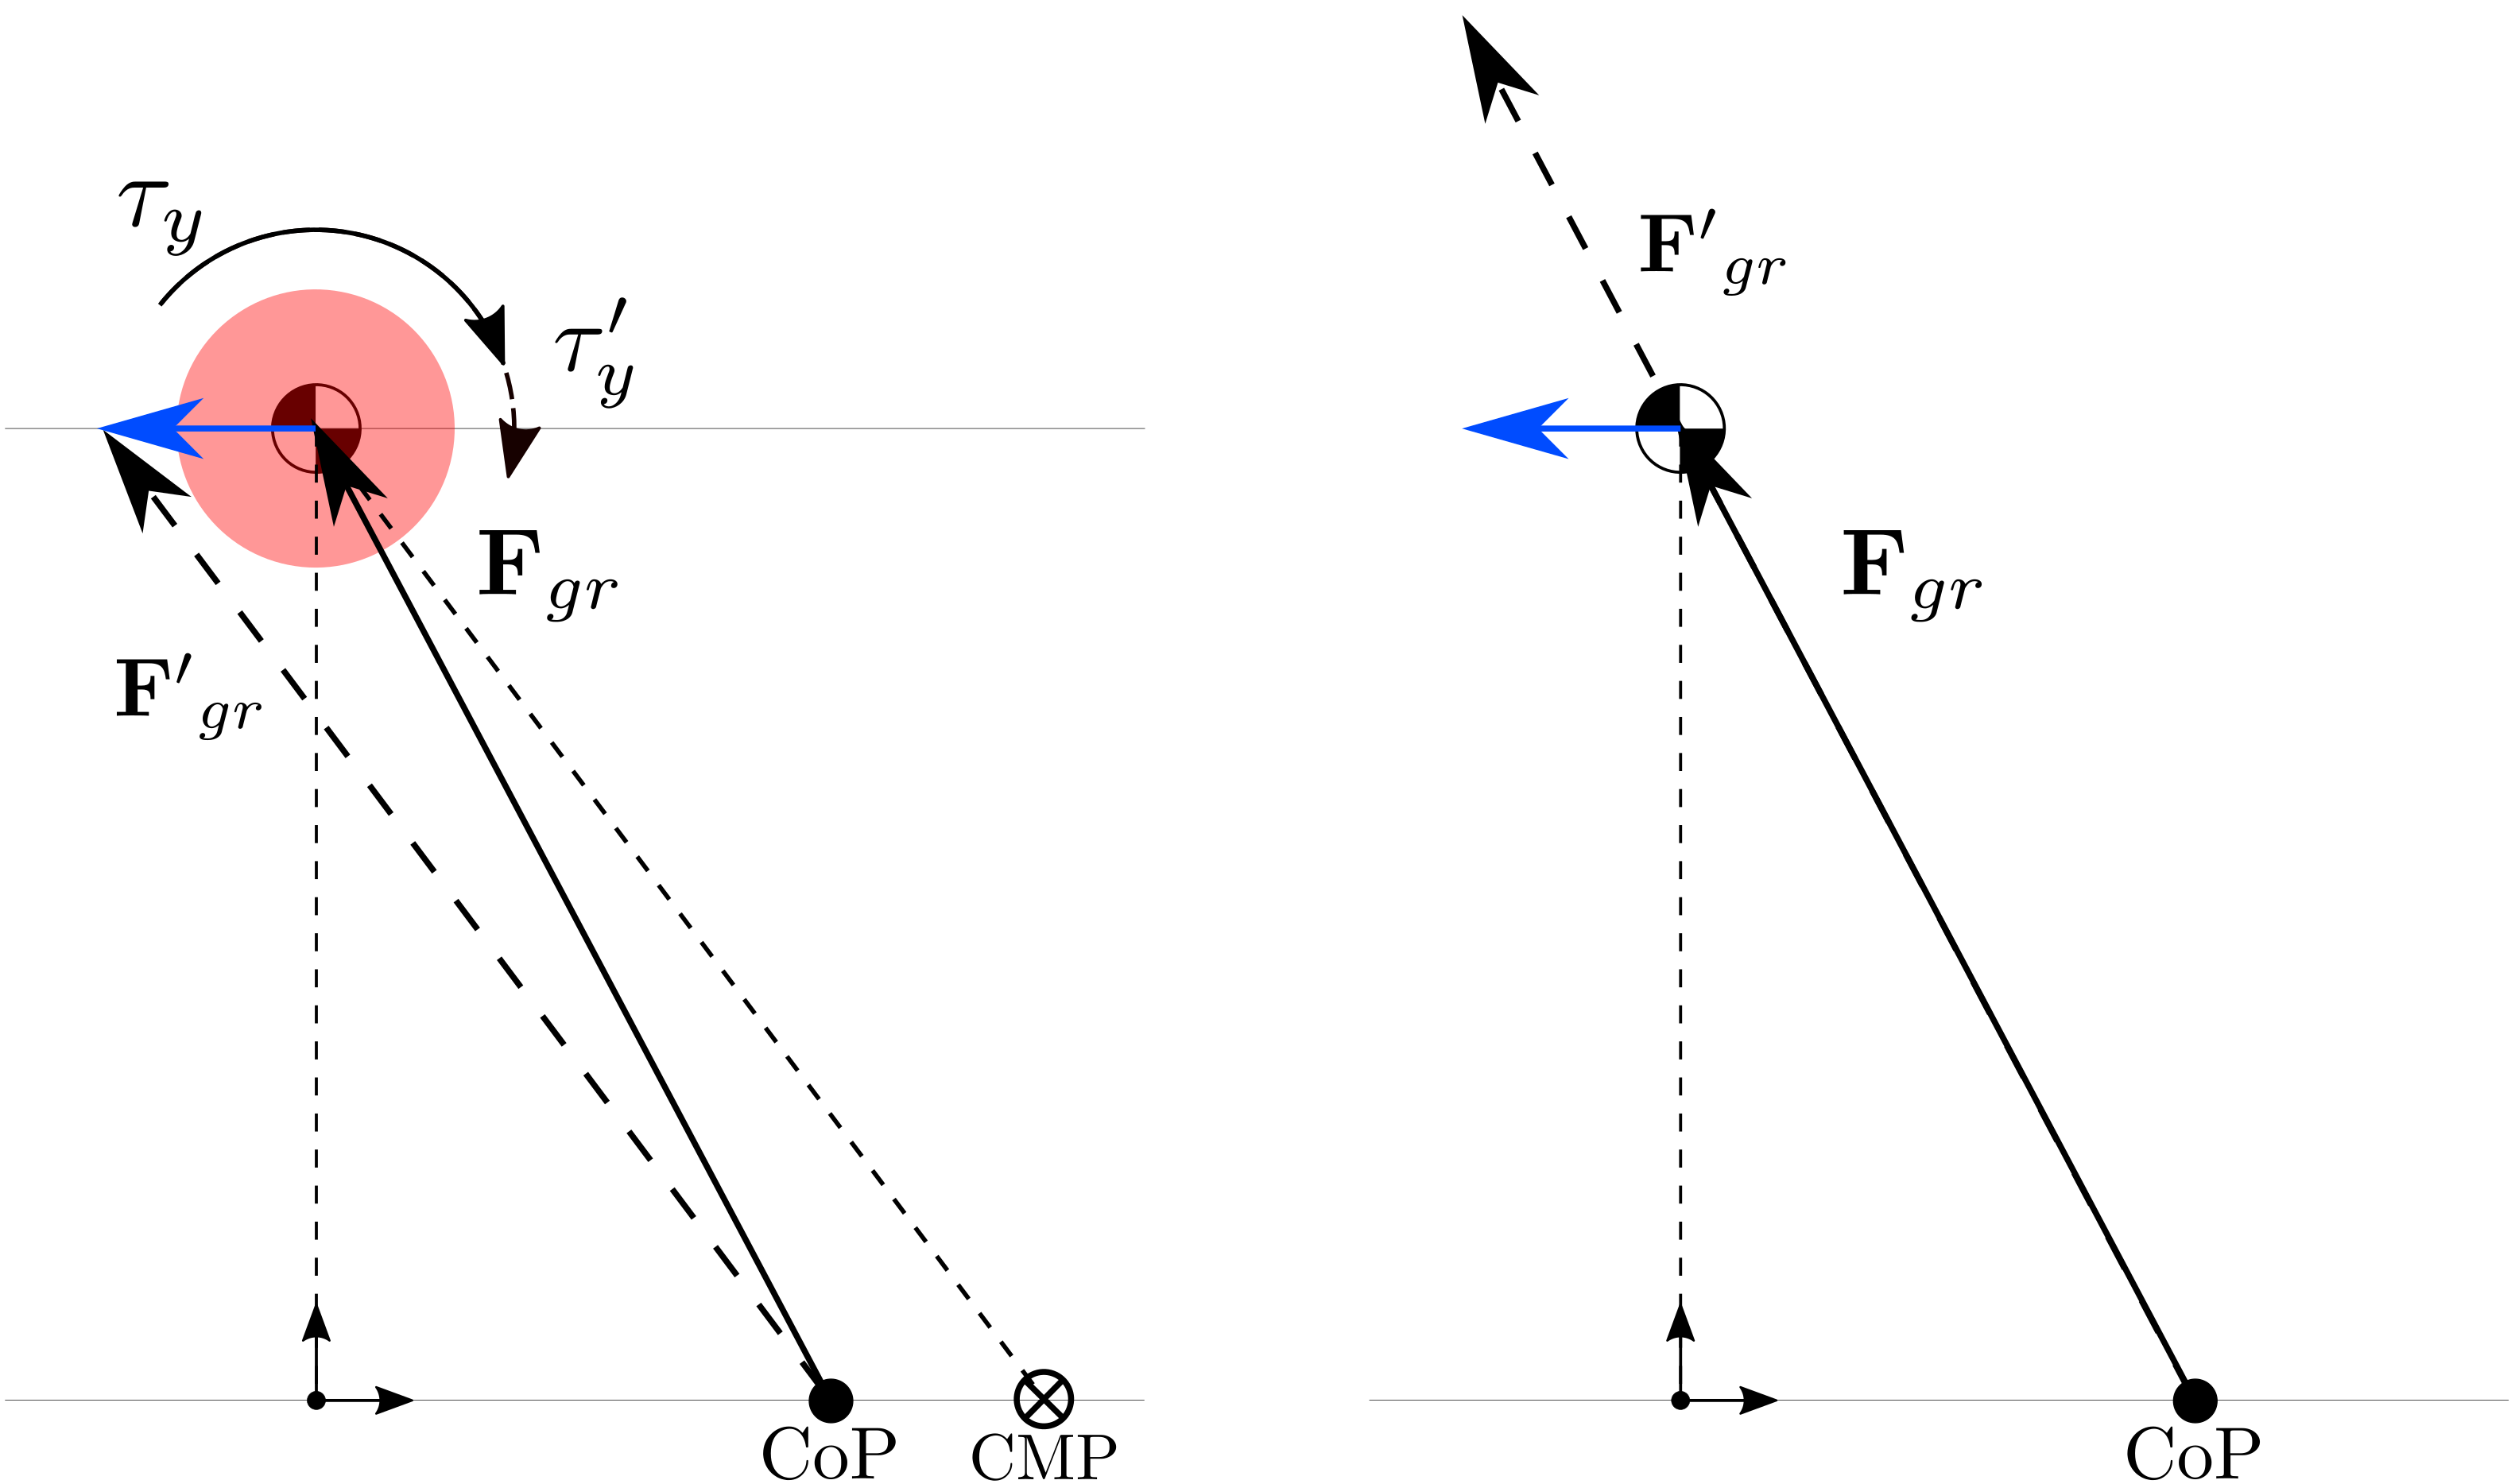
\includegraphics[width=3.2in]{modelvarzvsang2.png}
      \caption{Additional horizontal force on the CoM compared to the LIP model can be generated using angular momentum (left) and vertical motion (right). }
      \label{fig:angvsvarz}
\end{figure}

Related works  \cite{koolen2016balance}

This paper

The remainder of the paper is structured as follows.

\section{MODELS, BALANCE STRATEGIES \& CAPTURE}
One of the existing balance strategies if the CoP is saturated is the use of body angular momentum (see Fig. \ref{fig:angvsvarz}). The model to generate horizontal force is:
\begin{equation}
	\ddot{x} = g\frac{x}{z} + \frac{1}{m}\frac{\tau_y}{z}
\end{equation}

For the height varying point-mass, point-foot model, the following dynamics are considered:
\begin{equation}
	\ddot{x} = (g+\ddot{z})\frac{x}{z} 
	\label{eq:height}
\end{equation}

In this paper, we use the term capture region \cite{pratt2006capture} to describe the set of footholds, where balance can be achieved. Also, the capture point as introduced by Pratt et al is considered, only this is denoted as
\begin{equation}
	x_{cp,lip} = \sqrt{\frac{z_0}{g}}\dot{x}_0
\end{equation}
for comparison.
\section{THEORETIC CAPTURE REGIONS}
This section proposes bounds on the placement of the point-foot, where balance can be achieved. The dynamics of (\ref{eq:height}) are considered. For simplicity and comparison with the CP, $\dot{z}_0=0$ is considered.
\subsection{Unilateral Contact Constrained}
 Considering the constraint of unilaterality only, the capture region is bounded by the current position and the ballistic touch down point:
\begin{equation}
	x_{cp,unilateral} \in (0, x_{bal}], \quad \forall u>0, 
	\label{eq:xcpuni}
\end{equation}
where the ballistic touchdown point $x_{bal}=\sqrt{\frac{2z_0}{g}}\dot{x}=\sqrt{2}x_{cp}$ and $x_{cp,unilateral}$ is the capture point under unilateral contact constraint only. The proof for this region is given in \cite{koolen2016balance}.

\subsection{Addition of Height Constraints}
If to the unilateral constraint CoM height constraints are added, but limitations one forces are neglected, analytic capture regions can be derived. 

Preliminary, we temporally set $\dot{z}_0 \neq 0$ to calculate the influence of an impact on the CP. Considering an initial negative vertical velocity $\dot{z}_0<0$ that is driven to zero by a vertical impact, the influence on the CP is:
\begin{align}
	x_{cp,impact} &= \sqrt{\frac{z_0}{g}}(\dot{x}_0 + \frac{x_{cp,impact}}{z_0}\dot{z}_0)\\
	&=\frac{z_0}{\sqrt{z_0}-\dot{z}_0}\dot{x}_0,
\end{align}
where $x_{cp,impact}$ is the impact influenced capture point from an initial impact that results in $\dot{z}=0$.

Under a minimum height constraint, we can find a capture point from which the trajectory hits the constraint. We first let the mass follow the ballistic trajectory, after which it is stopped by the impact influenced capture point:
\begin{equation}
	x_{cp,\zmin} = x_{bal,\zmin} + x_{cp,impact}(\zmin, \dot{z}_{\zmin}),
	\label{eq:xcpzmincomp}
\end{equation}
where $x_{cp,\zmin}$ is the capture point over the minimum height constraint, $x_{bal,\zmin}$ the position from the ballistic trajectory at $\zmin$ and $x_{cp,impact}(\zmin,\dot{z}_{\zmin}$) is $x_{cp,impact}$ for that point.
The velocity at the moment the ballistic trajectory hits the constraint is:
\begin{equation}
	\dot{z}_{\zmin} = -\sqrt{2g(z_0-\zmin)},
\end{equation}
where $z_{min}$ is the minimum height constraint and $\dot{z}_{\zmin}$ is the vertical velocity at $z_{min}$. Using (\ref{eq:xcpzmincomp}), the capture point over the minimum height constraint reads as:
\begin{equation}
	x_{cp,\zmin} = (\sqrt{\frac{2\delta_{z_{min}}}{g}} + \frac{\zmin}{\sqrt{\zmin g}+\sqrt{2g\delta_{\zmin}}})\dot{x}_0,
\end{equation}
where $\delta_{\zmin}= z0-\zmin$.

Also under a maximum height constraint, an analytic capture point can be found. We consider a vertical impact by the leg at $x=x_0$, which is of such magnitude that the mass is exactly at maximum height if it is slowed down by gravity. After it is slowed down, we apply $x_{cp,lip}$. This point reads as:
\begin{equation}
	x_{cp,\zmax} =(t_{\dot{z}>0} + \sqrt{\frac{\zmax}{g}})\dot{x}_{0,I}
\end{equation} 
where $x_{cp,\zmax}$ is the capture point following the maximum height constraint, $t_{\dot{z}>0}$ is the time $\dot{z}>0$ and $\dot{x}_{0,I}$ is the initial velocity influenced by the impact. Note that the vertical impact that lets the mass just touch $\zmax$ is:
\begin{equation}
	\dot{z}_{I} = \sqrt{2g\delta_{\zmax}},
\end{equation}
where $\delta_{\zmax}=\zmax-z_0$. The capture point reads as:
\begin{align}
	x_{cp,\zmax} &= (\frac{\dot{z}_I}{g}+\sqrt{\frac{\zmax}{g}})(\dot{x}_0-\frac{x_{cp,\zmax}}{z_0}\dot{z}_I)\\
	&=\frac{z_0(\sqrt{2\delta_{\zmax}}+\sqrt{\zmax})}{\sqrt{g}(z_0 + 2\delta_{\zmax} + \sqrt{2\zmax \delta_{\zmax}})}\dot{x}_0.
\end{align}

We will show that the capture points $x_{cp,\zmin}$ and $x_{cp,\zmax}$ are also the outer bounds on the capture region.

\begin{lem}\label{lem:regionz}
Considering the dynamics of (\ref{eq:height}), $\dot{z}_0=0$, minimum height constraint $\zmin$ and maximum height constraint $\zmax$, $x_{cp,\zmin}$ and $x_{cp,\zmax}$ are the outer bounds on the capture region.
\end{lem}
\begin{proof}
For any $x_{cp}$, $x\dot{x}<0$ \cite{koolen2016balance} and $0>x_0>-x_{bal}$ (\ref{eq:xcpuni}). 
Note that $x \leq 0, \forall t$ and $x\rightarrow 0$ along any trajectory. From (\ref{eq:height}), and $z>0$ follows that any input $u$ will slow $\dot{x}$ down. Showing that $\frac{x}{z}\rightarrow 0, \forall t$ will proof that $u=0$ for the longest possible time $t$ will lead to the farthest $x_{cp}$, and a maximum $u$ on the earliest possible $t$ will lead to the closest $x_{cp}$. 

For $u=g$, $z$ remains constant and $\frac{x}{z}\rightarrow 0$. For $u>g$, $z$ will grow and $\frac{x}{z}\rightarrow 0$. If $u<g$, we can show with the derivative of $\frac{x}{z}$ that this is always increasing:
\begin{equation}
\frac{d\frac{x}{z}}{dt}= \frac{z\dot{x}-x\dot{z}}{z^2},
\end{equation}
where $x \leq 0$ and $z \dot{x} \geq 0$. Taking the extreme case $u=0$ leads to:
\begin{align}
	z\dot{x}-x\dot{z} &= (z_0 - \frac{1}{2}gt^2)\dot{x}_0 + (x_0 + \dot{x}_0 t)gt\\
	&= (z_0 +\frac{1}{2}gt^2)\dot{x_0} + x_0gt.
\end{align}
Noting that all terms are positive except for $x_0$, which has the largest negative value for $x_0=-x_{bal}$:
\begin{align}
	(z_0 +\frac{1}{2}gt^2)\dot{x_0} - \sqrt{\frac{2z_0}{g}}\dot{x}_0gt = (\sqrt{\frac{1}{2}g}t - \sqrt{z_0})^2,
\end{align}
which is always greater than zero for all $t$.
\end{proof}

In Fig. \ref{fig:capregion}, the discussed capture regions are visualized.
\begin{figure}[h]
      \centering
      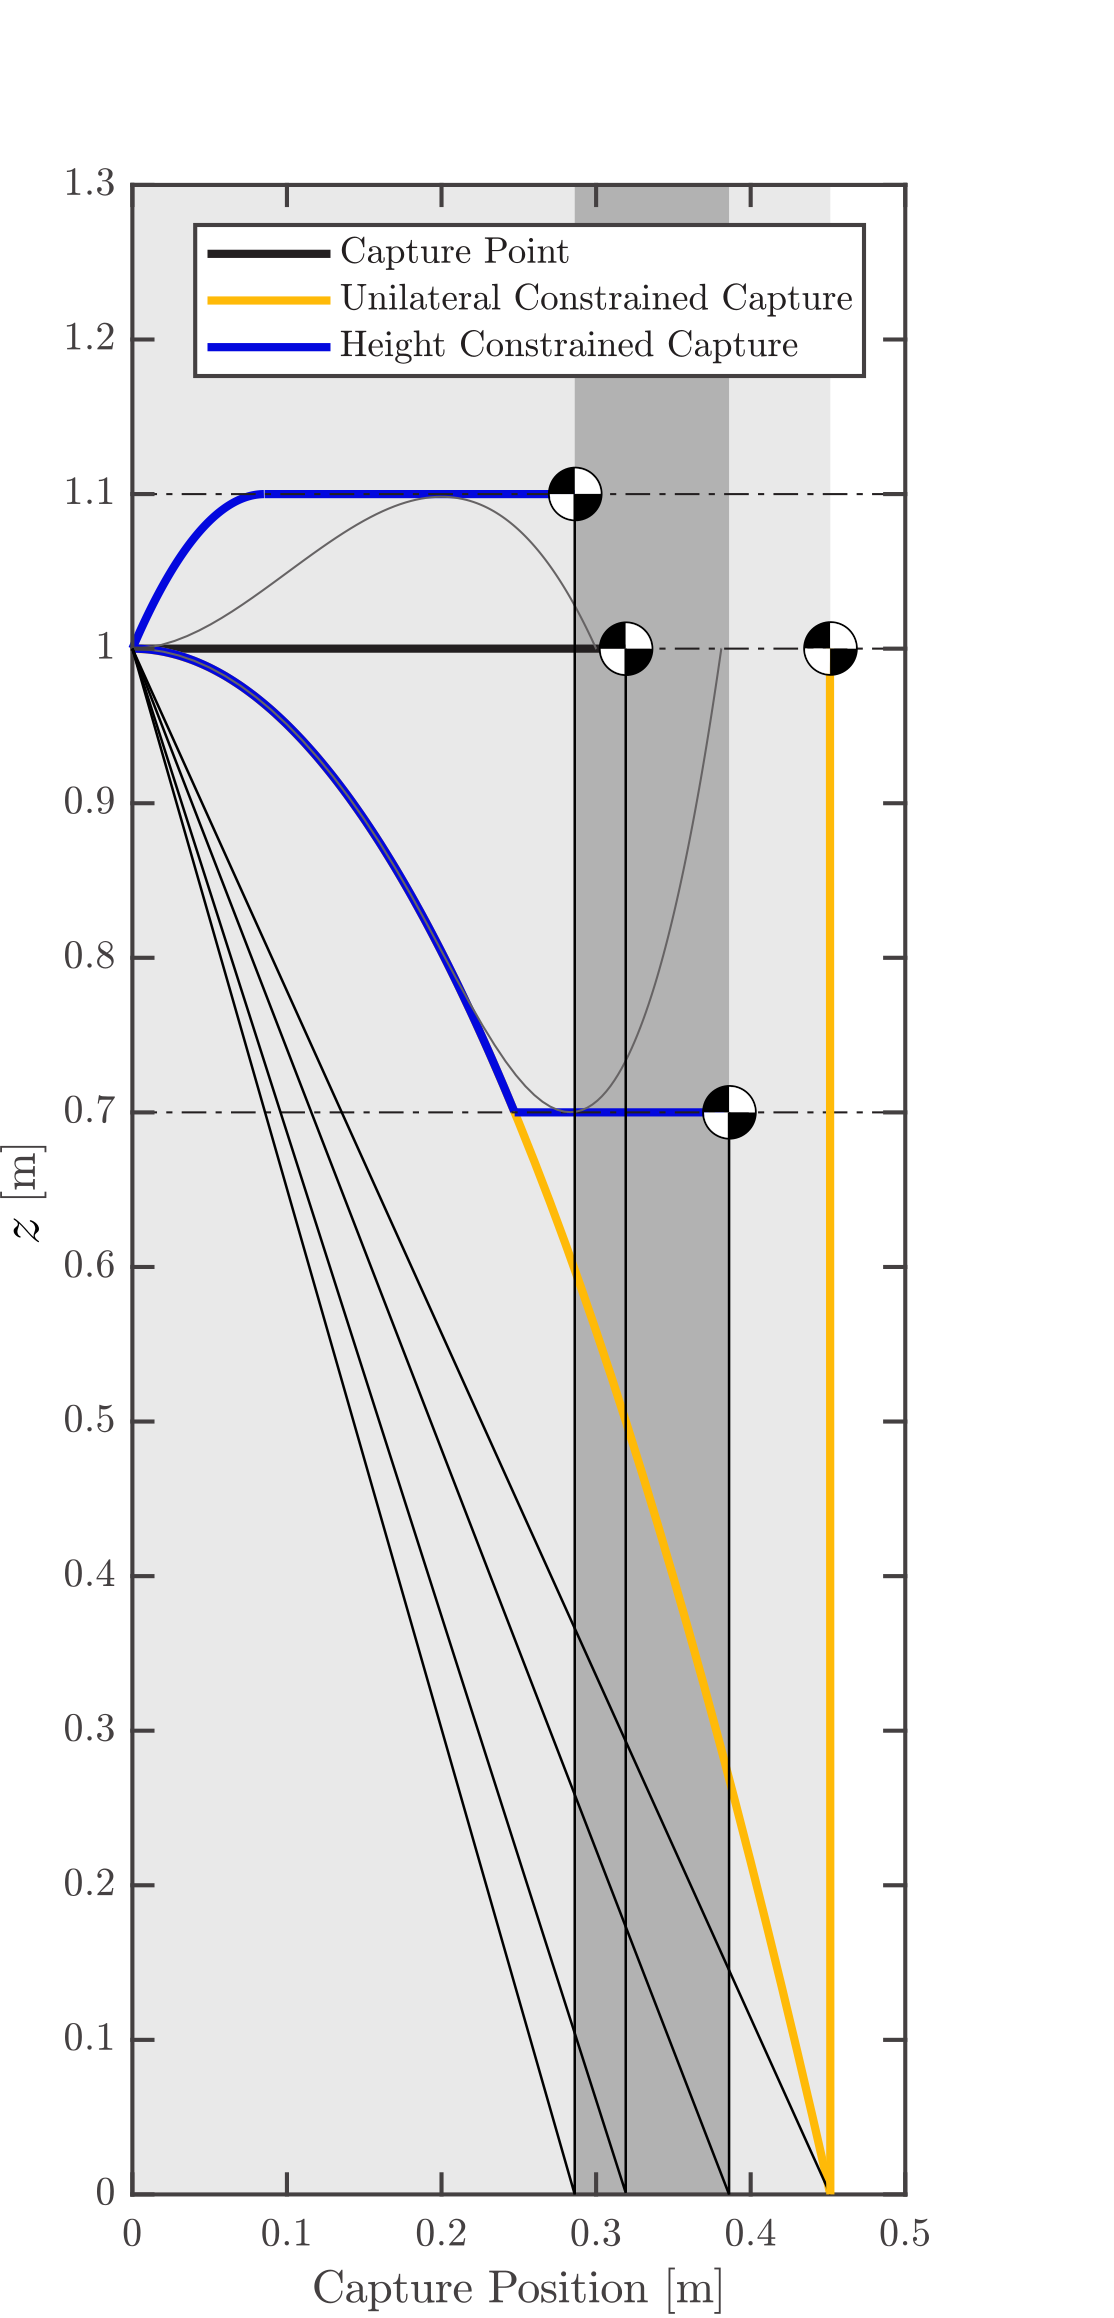
\includegraphics[width=2in]{CPLimits.png}
      \caption{Vizualisation of the capture regions. The light gray area shows the unilateral contact constrained region (\ref{eq:xcpuni}). The dark gray area shows the height constrained capture region (Lemma \ref{lem:regionz})  for $0.7<z<1.1$. The gray plots are made with the \textit{orbital energy controller} of \cite{koolen2016balance} and show that the final points are inside the region.}
      \label{fig:capregion}
\end{figure}
\subsection{Addition of Acceleration Constraints}\label{forcecapture}
If we add acceleration constraints on the dynamics (\ref{eq:height}), to take joint torque limits into account, an analytic solution for a capture point is not available anymore and needs to be solved numerically. 

In \cite{pratt2006capture,stephens2007humanoid,koolen2012capturability}, a bang-bang control law is used to regulate the angular momentum in the body of the model. Instead, we use a bang-bang control law for the input $u$.



\section{CAPTURABILITY COMPARISON}

\subsection{Effects of Angular Momentum}
Recap of \cite{pratt2006capture} bang-bang angular momentum controller
\subsection{Comparison with Vertical Motion}
\ref{forcecapture}
\section{PUSH RECOVERY ON NASA'S VALKYRIE}

\subsection{Control Law}

\subsection{Simulation Results}

\subsection{Hardware Results}
Box plot 3 cases: Default best recover, default fail, height controller best recover.

\begin{table}[h]
\caption{An Example of a Table}
\label{table_example}
\begin{center}
\begin{tabular}{|c||c|}
\hline
One & Two\\
\hline
Three & Four\\
\hline
\end{tabular}
\end{center}
\end{table}


   \begin{figure}[thpb]
      \centering
      \framebox{\parbox{3in}{We suggest that you use a text box to insert a graphic (which is ideally a 300 dpi TIFF or EPS file, with all fonts embedded) because, in an document, this method is somewhat more stable than directly inserting a picture.
}}
      %\includegraphics[scale=1.0]{figurefile}
      \caption{Inductance of oscillation winding on amorphous
       magnetic core versus DC bias magnetic field}
      \label{figurelabel}
   \end{figure}
   
\section{DISCUSSION AND FUTURE WORK}
\subsection{From Flywheel Model to Real Robot}
\subsection{3D Control}

\section{CONCLUSION}

A conclusion section is not required. Although a conclusion may review the main points of the paper, do not replicate the abstract as the conclusion. A conclusion might elaborate on the importance of the work or suggest applications and extensions. 

\addtolength{\textheight}{-12cm}   % This command serves to balance the column lengths
                                  % on the last page of the document manually. It shortens
                                  % the textheight of the last page by a suitable amount.
                                  % This command does not take effect until the next page
                                  % so it should come on the page before the last. Make
                                  % sure that you do not shorten the textheight too much.

%%%%%%%%%%%%%%%%%%%%%%%%%%%%%%%%%%%%%%%%%%%%%%%%%%%%%%%%%%%%%%%%%%%%%%%%%%%%%%%%



%%%%%%%%%%%%%%%%%%%%%%%%%%%%%%%%%%%%%%%%%%%%%%%%%%%%%%%%%%%%%%%%%%%%%%%%%%%%%%%%



%%%%%%%%%%%%%%%%%%%%%%%%%%%%%%%%%%%%%%%%%%%%%%%%%%%%%%%%%%%%%%%%%%%%%%%%%%%%%%%%

\section*{ACKNOWLEDGMENT}

The preferred spelling of the


%%%%%%%%%%%%%%%%%%%%%%%%%%%%%%%%%%%%%%%%%%%%%%%%%%%%%%%%%%%%%%%%%%%%%%%%%%%%%%%%

References are important to the reader; therefore, each citation must be complete and correct. If at all possible, references should be commonly available publications.


\bibliographystyle{IEEEtran}
\bibliography{IEEEabrv,IEEEexample}



\end{document}
